%%%%%%%%%%%%%%%%%%%%%%%%%%%%%%%%%%%%%%%%%
% University/School Laboratory Report
% LaTeX Template
% Version 2.0 (4/12/12)
%
% This template has been downloaded from:
% http://www.latextemplates.com
%
% License:
% CC BY-NC-SA 3.0 (http://creativecommons.org/licenses/by-nc-sa/3.0/)
%
% Original header:
%
% This is a LaTeX version of the sample laboratory report
% from Virginia Tech's copyrighted 08-09 CHEM 1045/1046 lab manual.
% Reproduction of this one appendix section for academic purposes
% should fall under fair use.
%
%%%%%%%%%%%%%%%%%%%%%%%%%%%%%%%%%%%%%%%%%

\documentclass{article}
\usepackage{graphicx}
\usepackage{mathtools}

\title{ELEC 302-81\\ Lab 1\\ Power in AC Circuits} % Title
% \author{John \textsc{Smith}} % Author name
\date{\today} % Specify a date for the report

\begin{document}

\maketitle

\begin{center}
  \begin{tabular}{l r}
    Date Performed: & January 14, 2013 \\
    Partners: & John Doe \\
              & Charles Pittman \\
    Instructor: & Dr. Weatherford
  \end{tabular}
\end{center}

\pagebreak

%\setlength\parindent{0pt} % Removes all indentation from paragraphs

\section{Introduction}
\begin{list}{}{}
  \item State the theoretical principles or concepts that this experiment is
    trying to prove.
  \item May also be to gain experience in using the lab equipment.
\end{list}

\section{Circuit Tested}
\begin{figure}[h]
  \begin{center}
    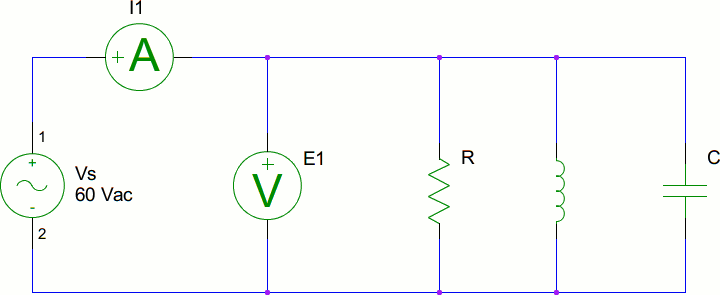
\includegraphics[width=.8\textwidth]{test_circuit}
  \caption{Parallel RLC Circuit Configuration}
  \label{test_circuit}
  \end{center}
\end{figure}

\begin{table*}[h]
  \begin{center}
    \begin{tabular}{ccc}
    \hline
    R & L & C \\
    \Omega & H & \mu{F} \\
    \hline
    1200 & 0.8 & --- \\ 1200 & 0.8 & 2.2 \\ 1200 & 0.8 & 4.4 \\
    1200 & 0.8 & 8.8 \\ 1200 & 1.6 & --- \\ 1200 & 1.6 & 2.2 \\
    1200 & 1.6 & 4.4 \\ 1200 & 1.6 & 8.8 \\
    \hline
    \end{tabular}
    \caption{RLC Values for circuit in Figure~\ref{test_circuit}}
    \label{calc_dat}
  \end{center}
\end{table*}

\section{Procedure}
\begin{list}{}{}
  \item Enough description that someone familiar with basic electrical
    measurements could reproduce the experiment.
  \item Sequential
  \item Paragraph form is usually preferred.
  \item Write in past tense.
  \item Do not just copy the instruction lists in the lab assignments.
  \item Learn to be brief
\end{list}

\section{Comparison with Theoretical}
\begin{list}{}{}
  \item Measured values versus what would be predicted by a theoretical
    analysis of the circuit performance.
  \item For example, compare the measured resistance of two resistors connected
    in series with R\(_1 + \)R\(_2\)
  \item Express comparison as a \%error.
\end{list}

\[\text{\%deviation} &=&
{{\text{measured} - \text{theoretical}} \over \text{theoretical}} \times \text{100\%}\]

\section{Conclusions}
What theoretical principle or concept did this experiment prove?

Within experimental error, this laboratory exercise has demonstrated that the
equivalent resistance of two resistors connected in series is equal to the sum
of the individual values.

\section{Calc}
\begin{table}[h]
  \begin{center}
    \begin{tabular}{cccccccccc}
      \hline
      R & L & C & I$_1$ & E$_1$ & P & \theta & S & Q & p.f. \\
      \Omega & H & \mu{F} & A & V & W & \deg & VA & VAR & \\
      \hline
      1200 & 0.8 & --- & 0.210 & 60 & 4.56 &  68.77 & 12.58 & 11.73 & 0.36 \\
      1200 & 0.8 & 2.2 & 0.164 & 60 & 4.56 &  62.48 &  9.86 &  8.75 & 0.46 \\
      1200 & 0.8 & 4.4 & 0.122 & 60 & 4.56 &  51.65 &  7.34 &  5.76 & 0.62 \\
      1200 & 0.8 & 8.8 & 0.076 & 60 & 4.56 &  -2.67 &  4.56 & -0.21 & 1.00 \\
      1200 & 1.6 & --- & 0.114 & 60 & 3.39 &  60.27 &  6.84 &  5.94 & 0.50 \\
      1200 & 1.6 & 2.2 & 0.075 & 60 & 3.39 &  41.06 &  4.50 &  2.96 & 0.75 \\
      1200 & 1.6 & 4.4 & 0.057 & 60 & 3.39 &  -0.50 &  3.39 & -0.03 & 1.00 \\
      1200 & 1.6 & 8.8 & 0.115 & 60 & 3.39 & -60.51 &  6.89 & -6.00 & 0.49 \\
      \hline
    \end{tabular}
    \caption{Calculated Data}
    \label{calc_dat}
  \end{center}
\end{table}
\section{Results}
\begin{table}[h]
  \begin{center}
    \begin{tabular}{cccccccccc}
      \hline
      R & L & C & I$_1$ & E$_1$ & P & \theta & S & Q & p.f. \\
      \Omega & H & \mu{F} & A & V & W & \deg & VA & VAR & \\
      \hline
      1200 & 0.8 & --- & 0.206 & 60.9 & 4.53 &  68.0 & 12.55 & 11.21 & 0.37 \\
      1200 & 0.8 & 2.2 & 0.158 & 60.9 & 4.56 &  60.9 &  9.62 &  8.19 & 0.49 \\
      1200 & 0.8 & 4.4 & 0.117 & 60.9 & 4.59 &  49.0 &  7.13 &  5.28 & 0.66 \\
      1200 & 0.8 & 8.8 & 0.081 & 61.0 & 4.65 &  -4.4 &  4.94 & -0.36 & 1.00 \\
      1200 & 1.6 & --- & 0.116 & 61.0 & 3.94 &  55.4 &  7.08 &  0.37 & 1.00 \\
      1200 & 1.6 & 2.2 & 0.079 & 61.0 & 3.96 &  32.8 &  4.82 &  2.55 & 0.84 \\
      1200 & 1.6 & 4.4 & 0.067 & 61.0 & 3.99 &  -6.6 &  4.09 & -0.46 & 1.00 \\
      1200 & 1.6 & 8.8 & 0.124 & 61.2 & 4.05 & -57.4 &  7.60 & -6.33 & 0.54 \\
      \hline
    \end{tabular}
    \caption{Experimental Data}
    \label{meas_dat}
  \end{center}
\end{table}

\end{document}
